%\todofilebegin{030\_sos\_model.tex}
%%%%%%%%%%%%%%%%%%%%%%%%%%%%%%%%%%%%%%%%%%%%%%%%%%%%%%%%%%%%%%%%%%%%%%%%%%%%%%
%%%%%%%%%%%%%%%%%%%%%%%%%%%%%%%%%%%%%%%%%%%%%%%%%%%%%%%%%%%%%%%%%%%%%%%%%%%%%%
%%%%%%%%%%%%%%%%%%%%%%%%%%%%%%%%%%%%%%%%%%%%%%%%%%%%%%%%%%%%%%%%%%%%%%%%%%%%%%



%
%%%%%

\subsubsection{The Need to Observe Locally at Run-Time}
%%%%%
%
%To be practically suited for exascale architecures, SOSflow is
%designed to collect and analyze information as close as possible to
%its source, and to accept metrics submitted from an arbitrary array of
%sources.
%
%SOSflow's in situ runtime design effectively parallelizes the execution of
%the observation system by scaling its capacity in direct proportion to
%the number of nodes observed.
%
%Each instance of SOSflow can operate independently and has the full
%suite of functionality, creating opportunities to alleviate
%coordination overhead when providing mechanisms for on-line feedback
%and control to massively parallel workflows.
%%%%%

\subsubsection{Monitoring Multiple Sources}
%
%Because many components can be operating concurrently on a single
%node, the monitoring solution must be capable of accepting
%information from multiple sources concurrently.
%%%%%

\subsubsection{Movement of Information}
%There are many methods to transport information between components of
%workflows.
%
%The optimal transport mechanism for a flow can depend on many factors:
%available hardware resources, topology of connected workflow
%components, total amount of information, size of data partitions,
%update frequency, data dependency relations, commonality of format,
%the expected useful lifetime of some data, etc.
%
%Information transport mechanisms are likely to differ not only between
%workflows, but also between runs of the same workflow on different systems.
%
%Workflow components can be coupled together by producing and consuming
%data files rather than using timely on-line communication, requiring
%SOSflow to provide an independent mechanism for information transport.
%
%Any two components of a scientific workflow are able to be connected
%in a way that makes the most sense for their particular exchanges,
%often multiple information transports are employed from end-to-end in
%a workflow.
%
%One transport technology can be used in drastically different ways
%within a workflow, such as with MPI's offering of efficient
%collectives, blocking synchronous point-to-point messages, and
%asynchronous one-sided communication.
%
%If the SOSflow routines endogenous to an instrumented component are
%communicating using the same mechanisms employed by the component
%itself, the desired SOSflow behavior cannot be guaranteed across all
%version of common data transport libraries such as MPI.
%
%SOSflow is designed to be minimally invasive and attempts to meet its
%own information transport needs without entangling or directly
%interfering with the workflow component's communications.
%
%Pervasive heterogeniety of technology, varying topology of connected
%components, deep configurability of workflows, and the inconsistent
%implementations of various transport technologies were each drivers
%for the independence of SOSflow from the coupling frameworks used to
%bind workflow components together.
%%%%%


\subsubsection{Modeling SOSflow as a General Solution}
%
%Independent pieces of embarassingly parallel simulations can be thought of
%as smaller isolated workflows within the context of their total experiment.
%
For any kind of scientific workflow, each single node's evolving state
is equally disposed to be a context for significant analysis, as much as
the whole of the simulation of allocation within which it runs.
%
This implies that even very small workflows, such as single-node simulations
running on a researcher's workstation, can utilize the full range of
SOSflow capabilities.
%%%%%


%-----------------------------------------------------------------------------

\subsection{Properties of the SOSflow Model}

%%%%%
%SOS's runtime framework is concieved of as eventually becoming an
%architectural addition to the general fabric of HPC clusters.
%
%SOS is intended to be a widely-integrated programmable middleware that
%evolves low-level optimizations over time, with a broad set of
%functionality that is available to all, especially developers and
%users of scientific workflows, regardless of job scale.
%
%During this early research phase, SOSflow runs in user space within
%the context of a single job's allocation.
%
%Operating in user space prevents native on-line datacenter-wide
%information aggregation and analysis, but has the significant benefit
%of making SOSflow deployable by any user in any context with support for its
%minimal dependencies.
%
%SOSflow imposes no major design or deployment requirements on workflows,
%given its effort to represent a general solution.
%
%The SOSflow platform targets extreme scales, but the design discipline
%required to offer its full suite of services in situ with minimal
%invasiveness means that SOSflow is well-adapted to provide coverage
%for smaller workflows, scaling effectively down to single-node runs.
%%%%%

%%%%%
%A non-trivial set of properties (Table \ref{tabledesign}) are required
%to meet the design goals of SOSflow.
%
%

\begin{table*}[t]
%% increase table row spacing, adjust to taste
\renewcommand{\arraystretch}{1.3}
\caption{SOSflow Design Properties and Means}
\label{tabledesign}
\centering
\begin{tabular}{|p{0.2\linewidth}|p{0.6\linewidth}|}
\hline %%%%%%%%%%%%%%%%%%%%%%%%%%%%%%%%%%%%%%%%%%%%%%%%%%%%%%%%%
%
\textbf{Scalable}
&
From one to millions of nodes
\\
%
%
\hline %%%%%%%%%%%%%%%%%%%%%%%%%%%%%%%%%%%%%%%%%%%%%%%%%%%%%%%%%
%
\textbf{Portable}
&
Many architectures and operating systems
\\
%
%
\hline %%%%%%%%%%%%%%%%%%%%%%%%%%%%%%%%%%%%%%%%%%%%%%%%%%%%%%%%%
%
\textbf{Easy To Use}
& 
Simple well-degined interfaces, minimal external software dependencies
\\
%
%
\hline %%%%%%%%%%%%%%%%%%%%%%%%%%%%%%%%%%%%%%%%%%%%%%%%%%%%%%%%%
%
\textbf{Multi-Purpose}
&
Utility not limited to any single component purpose, does not impose
a priori purposes for monitoring
\\
%
%
\hline %%%%%%%%%%%%%%%%%%%%%%%%%%%%%%%%%%%%%%%%%%%%%%%%%%%%%%%%%
%
\textbf{Concurrent With Workflow}
&
Runs at the same time as workflow in order to capture emergent
behavior
\\
%
%
\hline %%%%%%%%%%%%%%%%%%%%%%%%%%%%%%%%%%%%%%%%%%%%%%%%%%%%%%%%%
%
\textbf{In Situ Access}
&
Complete feature set available on-node, allowing distributed and
data-local analytics, feedback, and control
\\
%
%
\hline %%%%%%%%%%%%%%%%%%%%%%%%%%%%%%%%%%%%%%%%%%%%%%%%%%%%%%%%%
%
\textbf{Low Overhead}
&
Do not consume storage, bandwidth, or compute time wastefully, allow
system to be [de]activated dynamically
\\
%
%
\hline %%%%%%%%%%%%%%%%%%%%%%%%%%%%%%%%%%%%%%%%%%%%%%%%%%%%%%%%%
%
\textbf{Low Intrusion}
&
API calls should return rapidly, and users have means to exercise
control of storage vs. transport timing trade-offs
\\
%
%
\hline %%%%%%%%%%%%%%%%%%%%%%%%%%%%%%%%%%%%%%%%%%%%%%%%%%%%%%%%%
%
\textbf{Responsive}
&
Timeliness of replies should support application steering and global
state interrogation
\\
%
%
\hline %%%%%%%%%%%%%%%%%%%%%%%%%%%%%%%%%%%%%%%%%%%%%%%%%%%%%%%%%
%
\textbf{Can Dedicate Resources}
&
When available, make use of dedicated resources to avoid contention
\\

\hline %%%%%%%%%%%%%%%%%%%%%%%%%%%%%%%%%%%%%%%%%%%%%%%%%%%%%%%%%
%
\textbf{On-line Interactivity}
&
Handle control and introspection messages and replies while
workflow is running and SOSflow is continuously operating
\\
%
%
\hline %%%%%%%%%%%%%%%%%%%%%%%%%%%%%%%%%%%%%%%%%%%%%%%%%%%%%%%%%
%
\textbf{User-space}
&
Do not require administrative privileges for basic functionality
\\
%
%
\hline %%%%%%%%%%%%%%%%%%%%%%%%%%%%%%%%%%%%%%%%%%%%%%%%%%%%%%%%%
%
\textbf{Database}
&
Provide general-purpose SQL query access to data, and utilize
database technology internally
\\
%
%
\hline %%%%%%%%%%%%%%%%%%%%%%%%%%%%%%%%%%%%%%%%%%%%%%%%%%%%%%%%%
%
\textbf{HPC-friendly}
&
Take advantage of high-speed communication fabric unique to the
HPC environment.  Do not require components that are not suitable or
available for HPC
\\
%
%
\hline %%%%%%%%%%%%%%%%%%%%%%%%%%%%%%%%%%%%%%%%%%%%%%%%%%%%%%%%%
%
\textbf{Extensible}
&
Modular design and APIs to allow feature extension, configurable
behavior
\\
%
%
\hline %%%%%%%%%%%%%%%%%%%%%%%%%%%%%%%%%%%%%%%%%%%%%%%%%%%%%%%%%
%
\textbf{Global Information Space}
&
All information is contextualized and distinctly addressable, even
if not migrated off-node at run-time
\\
%
%
\hline %%%%%%%%%%%%%%%%%%%%%%%%%%%%%%%%%%%%%%%%%%%%%%%%%%%%%%%%%
\end{tabular}
\end{table*}



%

%%%%%


%
%  The key thing I want to do in this next section is
%  provide some clean abstract reasoningbehind the design choices
%  I made with SOSflow.
%
%  Such choices as:
%    - Fast socket-based in situ communication from app to daemon
%      to let applications push data in whenever it makes sense
%      for them to.
%    - Capturing and queue'ing updates to values to record
%      the full evolving history of a value with timing, so
%      developers can control when they interact with the daemon and
%      don't have to do it every time they make updates.
%    - Pervasive asynchronous messaging / transport within SOSflow
%         (we don't guarantee a QoS, but that allows for scaling
%          that allows for a decent QoS anyway.)
%    - GUIDs assigned to every value so SOSflow could be configured
%      such that (after initialization) it had ZERO information
%      transport impact.
%    - High-speed communication between daemons using site-optimized MPI
%    - Queryable data store in situ, to be able to run dist. analytics
%    - ...
%


\subsection{Model and Environment}
%%%%%
%For the purposes of further discussion, ''scientific workflow'' will imply 
%distributed instances of a workflow executing concurrently on two or more nodes.
%
%Considering the multi-node case will capture the important dimension
%of contention for shared network resources and the trade-offs that are
%encountered when optimization convergence is dependent on off-node
%information that is less reliably or quickly accessible than in situ
%data.
%
%Workflow execution environments provide the basis for comparing,
%validating, and selecting a particular means for achieving the SOSflow
%model.
%
%A following are some feature abstractions useful for reasoning about
%workflow execution environments:
%
%\begin{itemize}
%      %
%    \item \textbf{Available Memory}
%      %
%    \item \textbf{CPU Core Count}
%      %
%    \item \textbf{CPU Time}
%      %
%    \item \textbf{Node Count}
%      %
%    \item \textbf{Transport Bandwidth}
%      %
%    \item \textbf{Storage Bandwidth}
%      %
%\end{itemize}
%
%SOSflow has preconditioned properties for its general case (Table
%\ref{tabledesign}) and a model or combination of models should be
%employed that is suitable to meet each requirement, especially those
%regarding overhead and intrusiveness.
%
%These design requirements for SOSflow are indicators of the core
%functionality it ultimately provides for its users.
%
%There are a variety of information movement strategies (topologies)
%that might, singularly or cooperatively, meet the architectural
%conditions of SOS, and a subset of possible strategies is presented
%here.
%
%In order to stratify the models or combinations of them into a
%heirarchy of fitness, the impact on their resource-constrained
%operating environment should be considered.
%
%Each strategy intuitively has a dominant impact a different part of
%the environment, which is an indicator of its primary performance
%constraint:
%
%\todo[inline]{I don't like how this is set up, it seems like if
%I'm going to say these things I should have some numbers to back
%it up, and such a study is beyond the scope of this paper.}
%
%\begin{itemize}
%      %
%    \item \textbf{Distributed} - Transport bandwidth
%      %
%    \item \textbf{Centralized} - Transport bandwidth, storage bandwidth, node count
%      %
%    \item \textbf{Streaming Direct Messages} - Transport bandwidth, CPU Time, available memory
%      %
%    \item \textbf{On-line In Situ} - CPU Core Count, CPU Time, available memory
%      %
%    \item \textbf{Off-line In Situ} - Storage bandwidth, available memory
%      %
%\end{itemize}
%


%
%%%%%



%%%%%%%%%%%%%%%%%%%%%%%%%%%%%%%%%%%%%%%%%%%%%%%%%%%%%%%%%%%%%%%%%%%%%%%%%%%%%%
%%%%%%%%%%%%%%%%%%%%%%%%%%%%%%%%%%%%%%%%%%%%%%%%%%%%%%%%%%%%%%%%%%%%%%%%%%%%%%
%%%%%%%%%%%%%%%%%%%%%%%%%%%%%%%%%%%%%%%%%%%%%%%%%%%%%%%%%%%%%%%%%%%%%%%%%%%%%%

\section{Implementation}

%-----------------------------------------------------------------------------

\subsection{SOSflow}
%%%%%
%%%%%


%%%%%
Some accessory components are:
%
\begin{itemize}
    \item \textbf{sosd\_probe} - Collect real-time statistics from the daemon about
      its internal state and operating workload
      %
    \item \textbf{sosd\_stop} - Signal the SOSflow runtime to store its queues and
      safely shut down
      %
    \item \textbf{proc\_app} - Collect node runtime information from
      the /proc API on the node, submitting it to the daemon in the
      form of a publication
      %
    \item \textbf{demo\_app} - Benchmarking tool for testing SOSflow
      %
    \item \textbf{SOApy} - Python scripts for querying the SOS databases and plotting
      graphs from the results
      %
    \item \textbf{synthetic\_flow} - Tool for generating SOSflow-instrumented
      synthetic workflow of components using ADIOS+FlexPath
      that self-assemble into an arbitrary  user-specified DAG of
      data-dependent processing relations
      %
\end{itemize}
%%%%%

\subsection{SOSflow: Behavior}
%%%%%
%
At present, the ranks of sosd(listener) use a simple round-robin
selection method to pick their database target.
%
All the sosd instances split up the total numeric space from 0 to
UINT64\_MAX for use in assigning globally unique ids (GUIDs).
%
All entries in the SOSflow system from that point forward are, if
appropriate, assigned a GUID such that uniqueness and provenance is
preserved even if queries straddle multiple data stores, or all data
stores are eventually synthesized into a global store.
%%%%%

%%%%%


%%%%%
Once all of the sosd and sosa ranks are initialized and aware of each
other, they begin operating autonomously and no longer exchange global
collective messages -- all MPI messages are now point-to-point.
%
The sosd(listener) in situ daemons go into a loop listening to a
node-local TCP socket (specified by the SOS\_CMD\_PORT environment
variable) for messages from utilities or SOSflow-enabled source
applications.
%
The sosd(db) database daemons do not monitor any socket at this time,
but rather are contacted exclusively through their MPI communicator.
%
When an analytics module submits a query, it does not address the
database files directly, but sends its query to the sosd(db) instance
over MPI\_COMM\_WORLD and receives results back as an MPI message
which is transparently parsed into a row and column iteratable
(SOS\_results *) table.
%%%%%

%%%%%
On node, the sosd(listener) program accepts single messages at a time
and immediately services them, as far as the message sender is aware,
quickly responding with a simple ACK message or with the data that was
requested.  This behavior conforms to a very simple stateless protocol
that exists between the daemon and its on-node clients.
%%%%%


%%%%%
%

%%%%%

%%%%%
%
It is very uncommon to see the blocking socket transmission calls
within SOS\_announce() and SOS\_publish() take longer than 0.002
seconds, in any of our testing scenarios. Calls to the more frequently
used SOS\_pack() value storage/update routine create no noticable
overhead when not used in the innermost loops of intense computation,
often returning in less than 0.0001 seconds even for very large data
sets.
%
When a client first registers with the sosd(listener) during
SOS\_init(), the daemon will assign that client library a break of
GUIDs to manage internally, so that many different client activities
can be handled correctly with no need for immediate interaction with
the daemon.
%
When a client library runs out of GUIDs it simply pings the daemon and
asks for more.
%%%%%

%%%%%
The typical order of API calls in a client is:
%
\begin{enumerate}
      %
    \item SOS\_init();
      %
    \item SOS\_pub\_create();
      %
    \item SOS\_pack();
      %
    \item SOS\_announce();
      %
    \item SOS\_publish();\\
    \dots\\
    \dots\\
      %
    \item SOS\_finalize();
      %
\end{enumerate}
%%%%%


%%%%%
\begin{figure*}[!t]
\centering
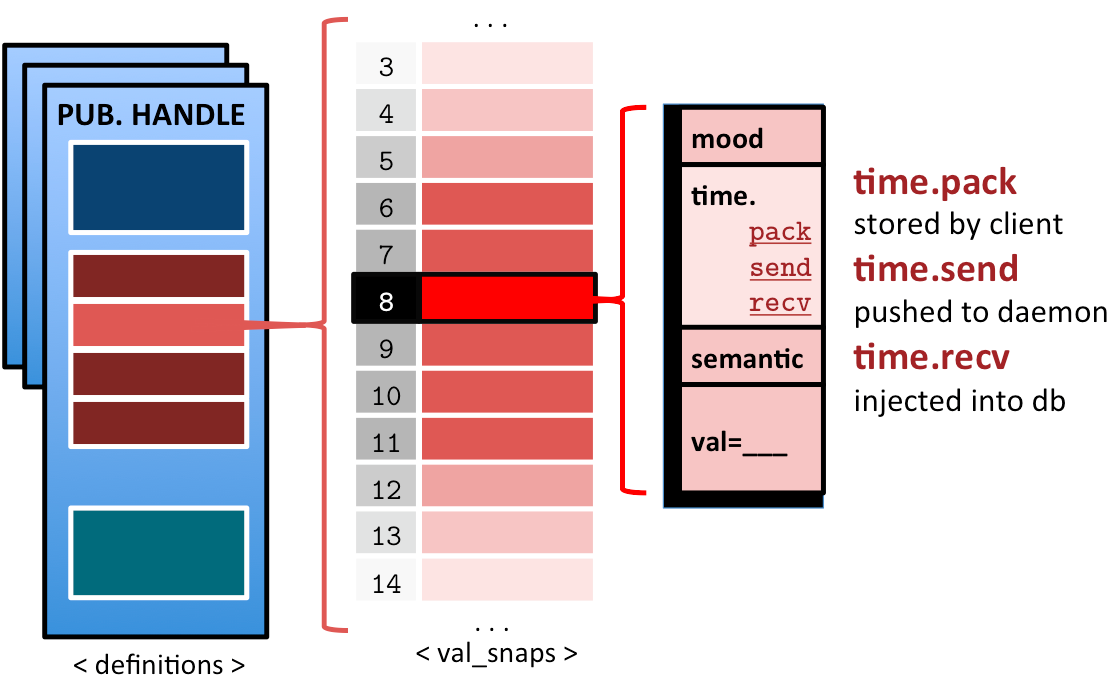
\includegraphics[width=5in]{images/val_snaps.png}
\caption{Complete History of For All Values, Including Metadata}
\label{fig_sim}
\end{figure*}
%%%%%

%%%%%
SOSflow is not a pure publish/subscribe system, the SOS\_announce()
function and its associated message type exist (for now) to seperate the
transmission of metadata apart from the transmission of the typically
more compact values stored in a pub.
%
Calling the SOS\_announce() function is entirely optional, though
never harmful, and good developer hygene in case it is not optional at
some point in the future.
%
If a pub handle has not been announced when it is passed to the
publish function, it with automatically recurse into the announce
function on your behalf.
%
Additionally, if you have added new value names, and not merely packed
updates to some previously announced values, the next time you
publish, those new value names will automatically be announced.
%%%%%

%%%%%
SOSflow is entirely thread-safe within the client application so long
as data elements are accessed only through the public API.
%
You could share a pub handle between two threads: the system is
designed to efficiently shield users from the complexity of managing
its state.
%
It is also designed to be as simple as possible without losing
flexibility.
%
When a value is packed into a pub handle, for the first time, that
effectively defines the value and configures it with a totally safe
set of metadata defaults.
%
If inspired to, a developer using SOSflow could then go render the
metadata more precise, though such noble pursuits are entirely
optional.
%
Data is thus defined to the system the same way it is updated in the
system, through the SOS\_pack() function.
%%%%%

%%%%%
The in situ sosd(listener) daemon does not keep track of applications,
and so does not know (or care) when they terminate.
%
The call to SOS\_finalize() provides a simple and clean way to release
SOS's internal memory objects and buffers, join any threads it may
have needed to spawn, and otherwise put things back how it found them
when SOS\_init() was called.
%
In the near future it is expected that SOS\_finalize() \textbf{will}
message the daemon, and so client applications should always make an
effort to call this function explicitly.
%%%%%

%%%%%
\subsection{SOSflow: Implementation}
%
\begin{itemize}
      %
    \item \textbf{Language}: C99
      %
    \item \textbf{External Requirements}:
      %
      \begin{itemize}
            %
          \item CMake
            %
          \item Pthreads
            %
          \item MPI
            %
          \item Sqlite3
            %
      \end{itemize}
      %
  \item \textbf{Key Source Files}: See Table 1.
    %
\end{itemize}
%%%%%

\begin{table}[!t]
%% increase table row spacing, adjust to taste
\renewcommand{\arraystretch}{1.3}
\caption{Key Source Files for SOSflow}
\label{tableexample}
\centering
\begin{tabular}{|c|c|}
\hline %%%%%%%%%%%%%%%%%%%%%%%%%%%%%%%%%%%%%%%%%%%%%%%%%%%%%%%%%
sos.h / sos.c & core functions of SOSflow\\
\hline %%%%%%%%%%%%%%%%%%%%%%%%%%%%%%%%%%%%%%%%%%%%%%%%%%%%%%%%%
sosd.h / sosd.c & SOSflow daemon\\
\hline %%%%%%%%%%%%%%%%%%%%%%%%%%%%%%%%%%%%%%%%%%%%%%%%%%%%%%%%%
sosa.h / sosa.c & SOS analytics core utilities\\
\hline %%%%%%%%%%%%%%%%%%%%%%%%%%%%%%%%%%%%%%%%%%%%%%%%%%%%%%%%%
sos\_debug.h & Debugging off / on (level) knobs\\
\hline %%%%%%%%%%%%%%%%%%%%%%%%%%%%%%%%%%%%%%%%%%%%%%%%%%%%%%%%%
demo\_app.c & Synthetic app for profiling SOSflow\\
\hline %%%%%%%%%%%%%%%%%%%%%%%%%%%%%%%%%%%%%%%%%%%%%%%%%%%%%%%%%
sosd\_cloud\_mpi.c & Off-node transport, coordination\\
\hline %%%%%%%%%%%%%%%%%%%%%%%%%%%%%%%%%%%%%%%%%%%%%%%%%%%%%%%%%
sosd\_db\_sqlite.c & Database operations\\
\hline %%%%%%%%%%%%%%%%%%%%%%%%%%%%%%%%%%%%%%%%%%%%%%%%%%%%%%%%%
\end{tabular}
\end{table}


%-----------------------------------------------------------------------------
\subsection{SOSa : Analytics}

%%%%%
SOSflow supports online query and analysis of the information that is
published into it.
%
Users of SOS are able to quickly write their own analytics modules
building by expanding from the provided templates.
%
When the sosd daemons are brought online, analytics modules are also
activated using MPMD syntax to add them to the daemon's mpirun
invocation.
%
Multiple analytics modules can be launched at once, so long as they
define unique SOSA\_MODULE\_COLOR values.
%
These unique 'colors' are used to split each analytics group into its
own communicator so the analytics codes can benefit from the HPC
resources of the job allocation to perform their work without engaging
with any other parts of SOSflow.
%
Queries are written in the dialect of SQL supported by the daemon, and
in the current case this is the fairly standard version in Sqlite3.
%
The query submitted as a string in a character array, and a special
(SOS\_results *) object is returned:
%%%%%

%%%%%
\begin{lstlisting}[frame=single, basicstyle=\small]
typedef struct {
    SOS_runtime *sos_context;
    int          col_max;
    int          col_count;
    char       **col_names;
    int          row_max;
    int          row_count;
    char      ***data;
} SOSA_results;

SOSA_results *results;                                                                                                                       
SOSA_results_init(SOS, &results);
char *query =
    "SELECT "
       "max(rowid), "
       "time_pack, "
       "time_recv "
    "FROM tblvals;";

SOSA_exec_query(query, results);

SOSA_results_output_to(fptr,
    results,
    "latency",
    SOSA_OUTPUT_W_HEADER);
\end{lstlisting}
%%%%%

%%%%%
There are utility functions to reset and destroy SOS\_results objects,
output them as CSV tables of JSON object lists, etc.
%
The full API for developers of analytics modules is available in the
sosa.h header file.
%%%%%

%%%%%
Queries are submitted to an aggregator daemon that your analytics
module is targeting.
%
sosd(db) ranks and sosa modules can be pinned to the same physical
node together at invocation, and analytics modules will favor the
sosd(db) rank they share a node with in order to enable fast in-memory
messaging rather than sending query results across the shared network
resources.
%
Queries are entirely arbitrary, and are allowed to examine the full
scope of data that has been submitted to the SOSflow runtime, from
whatever source derived.
%
At this time there are no security measures to prevent analytics
modules from accessing specific regions of the data, since all of the
data available in the database will have come from a user's own
applications.
%
This is a section of the SOSflow development that is relatively novel,
and has not been implemented with much optimization in place.
%
When a query is executed it locks the database to prevent other
threads from writing to it.
%
It is possible to write very inefficient queries that tie up the
database and create latency in the asynchronous queues.
%
Avoiding such issues is an exercise left to developers at this time,
though re-architecting this component of SOSflow is a high priority
for the next phases of its maturation.
%%%%%



%%%%%%%%%%%%%%%%%%%%%%%%%%%%%%%%%%%%%%%%%%%%%%%%%%%%%%%%%%%%%%%%%%%%%%%%%%%%%%
%%%%%%%%%%%%%%%%%%%%%%%%%%%%%%%%%%%%%%%%%%%%%%%%%%%%%%%%%%%%%%%%%%%%%%%%%%%%%%
%%%%%%%%%%%%%%%%%%%%%%%%%%%%%%%%%%%%%%%%%%%%%%%%%%%%%%%%%%%%%%%%%%%%%%%%%%%%%%

%
%   NOTE: It gets pretty loose from here on... this needs to be condensed
%         and focused A LOT.
%


%-----------------------------------------------------------------------------

\subsection{Semantic Markups and On-line Reasoning}
%%%%%
By defining a stable meaning for observations to be
set off against, the meaning in the codes, the partially summed yet
variously disanalogous sets of observed metrics from a system as a
whole, can be mapped over each other according to a set of organizing
principles that both are individually, and become corporately, an
invariant for that particular complex computation.
%
It doesn't only matter that something is a double precision floating
point, it matters that it holds a measure of time, and it matters that
it's the time something stopped, rather than a simple sample.
%
It doesn't only matter that a process uses a lot of threads, it
matters that it is running well on a machine with a lot of thread
processing cores.
%
It isn't obviously significant for a task to be parameterized by an
auto-tuning algorithm to increase the rate of one of its outputs
rather than other targets, like reducing node memory use, or
increasing the degree of paralellism, unless it is clear that
\textit{something in its output} is being consumed at a great rate
through unsaturated network connections.
%
\textbf{It is only by observing all of these meaningful
  \textit{natures}, \textit{purposes}, and \textit{activities}, that
  the complexity can be properly reasoned about, that the \textit{true
    figure of performance} can be revealed.}
%
It is only with a proper run-time and annotation framework that this
reasoning can take place in a computationally feasible way.
%%%%%

%%%%%
In a very basic sense, so long as it holds that with a certain input a
particular result will be output the same, there is something else
unchanging about a simulation, however it has been tuned or allocated
or configured for a run: the meaning of what happened.
%
Whether a simulation is executing as a single process on a single
node, or billions of independent tasks in a cloud computing
environment, the meaning of what is being computed holds the
same.
%
Though this point may seem fine if not obtuse in this context, the
concept of \textit{invariant meaning} is central to a properly useful
Workflow Performance Model: It must be a Semantic Performance Model.
%%%%%

%%%%%
At extreme scales, online detection and attribution of meaningful
variability in the performance of a scientific workflow will simply
\textit{require} well-annotated metadata to facilitate apples to
apples comparisons driven by unsupervised machine learning rather than
a priori developer knowledge or slow offline centralized analysis.
%
Offline big data analytics can help discover the features of
workflows that will allow helpful runtime predictions like
precursors to hardware failures, shared resource consumption, and
predictions of I/O requirements for scheduler optimization.
%
Once the features are mapped out and a model is developed that
facilitates complex event classification, it will need to be handed
off to an in situ runtime that can efficiently detect information
that fits the model.
%
Having consistent semantic annotation will facilitate complex event
detection.\todo[inline]{Duh.}
%
In the face of wild performance variance across byzantine parameter
spaces, hardware allocations, software libraries, and dynamic
interactions, this kind of meaning invariance is the only ground
truth, the only practical measure of what has been observed.
%
With meaning invariance properly worked into the observation and
analytics structure, real-time systems will be able to efficiently
discover, annotate, share, and potentially even optimize a code's
sensitivity to a particular cluster or allocation, its propensity for
creating and propagating performance variability into other unrelated
parts of the system, and then finally pinpoint the lower-level
software mechanics giving rise to the higher level phenomenon.
%%%%%

%-----------------------------------------------------------------------------

\subsection{Levels of Description and "The View from Anywhere"}
%%%%%
Not wanting to limit \textit{a priori} what component or layer of the
workflow \textit{is allowed to be interesting} during the analysis of
performance, the SOS workflow performance model flourishes when
populated by a diversity of information sources, each providing
metrics with tailored metadata, logical events like notes about things
happening inside the simulation they are running, and concrete events
-- all arriving in real-time from many different layers of activity in
a workflow:
%
\begin{itemize}
      %
    \item Workflow
      %
    \item Simulation
      %
    \item Application
      %
    \item Algorithm
      %
    \item Libraries
      %
    \item Environment
      %
    \item Developer Tools
      %
    \item Operating System
      %
    \item Node Hardware
      %
    \item Network
      %
    \item Enclave
      %
    \item Cluster
      %
    \item Epoch
      %
\end{itemize}
%%%%%

%%%%%
Each of these layers constitutes a level of description for the
overall system performance, and the performance of any component is a
composite of slices through any layers that component is participating
in or contingent on.
%
It becomes a tantalizing possibility that events and metrics stored in
SOS for a very narrow end-user purpose wind up supporting critical
inferences used to discover patterns and features of system-wide
utility.
%
If a developer finds she can get some benefit by using the SOSflow
toolkit for a once-off research project, the metrics that are then
even \textit{accidentally} contributed might turn out to have been
unpolished research gems hiding in tomorrow's data stores.
%%%%%

%%%%%
Metrics from multiple layers can be correlating to yield interesting
perspectives on the observed performance of specific software
components.
%
As a trivial example, if something at the Simulation layer produces data
representing the evolution of a data set over N seconds of simulated
time, and the Application layer requires M seconds of real-world
computation to yield that data, the relationship between N and M could
be a valid performance metric to report, compare across runs,
calculate real-dollar-cost to compute, or attempt to generally
optimize through parameter convergence.
%
A key takeaway here is: \textit{The particular purpose for gathering
  that data does NOT need to be known in advance}, sampling would not
need to be programmed into the application by hand every time a
researcher or performance tuning engine asked a question, rather,
on-demand queries could be run to discover such correlations and
features of performance at any time, or \textit{even in real-time} as
fresh data is flowing in.
%
It is also important to note that components of a layer not only can
contribute metrics, they (and other components at that layer) are
targets for feedback and control.
%%%%%

%-----------------------------------------------------------------------------

\subsection{Semantics}

All information that is gathered by the monitoring system should be
annotated as richly as possible to maximize its usefulness when
performing analytics.
%
Hand-annotated codes will have the most to offer an analytics engine,
values that are tracked will be able to carry a full spectrum of
high-level tags that express what that data means and what could be
expected of it, in structures preserving some human programmer or
user's understanding.
%
Capturing this metadata using semantic markups with action-grounded
significance has the benefit of their being compatible with
unsupervised machine-learning tests for significance and other
advanced analysis techniques that will ultimately be able to converge
on outcomes desirable to the human developers and users of the system.
%%%%%

%%%%%
Not every bit of data has to be surgically annotated for it to be of
benefit.
%
Any episodic performance measurement, such as run-time TAU
instrumentation and results, can also be injected into the SOSflow
engine, and the SOSflow runtime is able to differentiate from
information pushed directly by a layer, and information that is being
captured by finer-grained middleware tools that are only equipped to
signify generic matters of fact.
%%%%%

%%%%%
Semantic information is local to the pub handle created by a source
that is contributing to SOSflow.
%
Sources can create multiple pubs to distinctly represent potential
compound or complex roles.
%
Pubs carry their own pub-wide semantic markups, including the origin
layer, a role within that layer, and information about the node that
the source process is running on.
%
Semantic markups are then nested inside of the pub handle, as each
value that is pushed into the SOSflow system through a pub handle also
comes with a rich set of high-level semantic tags that stay affiliated
with it over time, and various ephemeral notions to color the rigid
meaning invariance with motivating indicators of changes in state,
such as the \textit{mood} of a value, which can be: DEFAULT, GOOD,
BAD, UGLY.
%
The ephemeral indicators are mere hints, motivators, not themselves
signifiers of meaning but more the glue between meanings revealed by
the coocurrence of change.
%
Sometimes it matters less what changed into what, than that something
changed at all.
%%%%%

While deep off-line data analytics can reveal \textit{unforseen
  correlations} between various aspects of the workflow or the data
set it is operating over, the interest in real-time analytics and
performance tuning gives value to expressing relationship hints
between values tracked by the system.
%
These hints can be used to direct in situ analytics efficiently, to
narrow the parameter space into something tractable without
interfereing with the principle computational load of a given
node.
%
Expressed relationship hints are a double-edged sword, as one of the
draws of the performance model is that nobody has to know the big
picture in order to get some value out of it.
%
Rather than call them relationship \textit{rules} we say
\textit{hints} and suggest that unless someone really knows what
they're looking for, such as when they write an online analytics
module for their own code, the hints functionality can be safely
ignored.
%
When one's analytics are looking to identify specific deviations from
predictable expectations; anything that can be overtly identified as
an expectation for a value can be used to narrow the search space when
doing unsupervised machine learning over gathered workflow performance
data.
%
Such accessory features are supported but not required, or even truly
emphasized.
%%%%%

%-----------------------------------------------------------------------------

\subsection{The Utility a Comprehensive Semantic Performance Model}

%%%%%
At this point it is safe to leave it to the reader's imagination to
ponder the possible utility of a mature Semantic Performanice Model /
Workflow Performance Model.
%
Especially given that there is an extant implementation of it that
functions with relative efficiency and is capable of operating online
and in user space on today's commodity HPC hardware.
%
The exascale architectures will likely prove even more effective
hosts: Their incredible computational density and scale has proven
difficult to completely saturate with work that is purely organic to
any given problem at hand, so there will likely be plenty of available
computational resources to direct towards these higher-level systems.
%%%%%

%%%%%
Some specific immediate perks would be enhancements to:
%
\begin{itemize}
      %
    \item \textbf{Attribution}: Point the blame at the offending job
      or shared resource.
      % 
      Developers don't always know their own code so well, or how it
      will interact with a total system, so capturing from a wide
      array of sources will help eliminate the guessing game when it
      comes time to grab the pitchforks.
      %
    \item \textbf{Accuracy}: If you've got data showing consistent behavior on
      certain allocations, and bad behavior when certain hardware resources
      get involved, you've got a better sense about what part of your
      fate you can control, about what variation is yours, and what comes
      from the Lord.
      %
    \item \textbf{Resource Requirement Prediction}: 2 + 2 isn't always
      4 when it comes to guessing about the perturbation of processes
      interacting in dynamical systems.
      %
      Being aware of each other's presence through shared real-time
      self-reporting will allow applications to adapt themselves and
      administrators to preemptively allocate to promote positive
      disruption of learned negative performance patterns.
      %
    \item \textbf{Automated Component Performance Tuning}: Nobody
      wants conflicting optimizer purposes, and having them working
      from a global perspective will need to show where the true
      systemic hotspots really are, and not depend on an individual
      developer being a total system expert or a selfless
      non-optimizer.
      %
    \item \textbf{Intelligent Compiler Hints}: Anything that is learned from all
      this richly annotated performance data can ultimately be tied back
      into intelligent compilers and IDE's.
      %
      That way a new hire doesn't have to burn 1,000,000 hours of
      allocation to learn that they've just re-created the exact code
      pattern or data structure that led to last year's round of
      layoffs and funding cuts.
      %
    \item \textbf{Intelligent Job Scheduling}: Because ``optimum job
      scheduling'' is not a univocal term.
      %
\end{itemize}
%%%%%


%\todofileend{030\_sos\_model.tex}
